%%%%%%%%%%%%%%%%%%%%%%%%%%%%%%%%%%%%%%%%%%%%%%%%%%%%%%%%%%%%%%%%%%%%%%%%
%    INSTITUTE OF PHYSICS PUBLISHING                                   %
%                                                                      %
%   `Preparing an article for publication in an Institute of Physics   %
%    Publishing journal using LaTeX'                                   %
%                                                                      %
%    LaTeX source code `ioplau2e.tex' used to generate `author         %
%    guidelines', the documentation explaining and demonstrating use   %
%    of the Institute of Physics Publishing LaTeX preprint files       %
%    `iopart.cls, iopart12.clo and iopart10.clo'.                      %
%                                                                      %
%    `ioplau2e.tex' itself uses LaTeX with `iopart.cls'                %
%                                                                      %
%%%%%%%%%%%%%%%%%%%%%%%%%%%%%%%%%%
%
%
% First we have a character check
%
% ! exclamation mark    " double quote  
% # hash                ` opening quote (grave)
% & ampersand           ' closing quote (acute)
% $ dollar              % percent       
% ( open parenthesis    ) close paren.  
% - hyphen              = equals sign
% | vertical bar        ~ tilde         
% @ at sign             _ underscore
% { open curly brace    } close curly   
% [ open square         ] close square bracket
% + plus sign           ; semi-colon    
% * asterisk            : colon
% < open angle bracket  > close angle   
% , comma               . full stop
% ? question mark       / forward slash 
% \ backslash           ^ circumflex
%
% ABCDEFGHIJKLMNOPQRSTUVWXYZ 
% abcdefghijklmnopqrstuvwxyz 
% 1234567890
%
%%%%%%%%%%%%%%%%%%%%%%%%%%%%%%%%%%%%%%%%%%%%%%%%%%%%%%%%%%%%%%%%%%%
%
\documentclass[12pt,a4paper,final]{iopart}
\usepackage[letterpaper]{geometry}
\newcommand{\gguide}{{\it Preparing graphics for IOP journals}}
%Uncomment next line if AMS fonts required
\usepackage{iopams}  
\usepackage{graphicx}
\usepackage[breaklinks=true,colorlinks=true,linkcolor=blue,urlcolor=blue,citecolor=blue]{hyperref}
%\usepackage[T1]{fontenc}
%\usepackage{alltt}
%\usepackage{underscore}

%% Choose Font %%
%\usepackage{fontspec}
%\setmainfont{Fontin}
\usepackage{libertine}
\usepackage{graphicx}

\usepackage[colorlinks=true]{hyperref}

\begin{document}

\title[Information for DOE Report]{Information for DOE Report}
	
\author[cor1]{Shih-Kai Lin}
\address{Colorado State University}
\ead{\mailto{Shihkai.Lin@colostate.edu}}


%\begin{abstract}
%This document describes the  preparation of an article using \LaTeXe\ and 
%\verb"iopart.cls" (the IOP \LaTeXe\ preprint class file).
%This class file is designed to help 
%authors produce preprints in a form suitable for submission to any of the
%journals published by IOP Publishing.
%Authors submitting to any IOP journal, i.e.\ 
%both single- and double-column ones, should follow the guidelines set out here. 
%On acceptance, their TeX code will be converted to 
%the appropriate format for the journal concerned.
%
%\end{abstract}

%Uncomment for PACS numbers title message
%\pacs{00.00, 20.00, 42.10}
% Keywords required only for MST, PB, PMB, PM, JOA, JOB? 
%\vspace{2pc}
%\noindent{\it Keywords}: Article preparation, IOP journals
% Uncomment for Submitted to journal title message
%\submitto{\JPA}
% Comment out if separate title page not required
%\maketitle

\vspace{\baselineskip}
This document summarizes the work I have done in the past year for the DOE report, starting with DUNE and followed by NO$\nu$A.

\tableofcontents

\clearpage
\vspace*{\fill}
\begin{Huge}
\center{\textbf{Work in 2016}}
\end{Huge}
\vspace*{\fill}
\clearpage

\section{Work in 2016}

\subsection{DUNE}

\subsubsection{Tuning the Photon Detector Thresholds for the 35-ton Data Taking}\hspace*{\fill}\\
During my February stay at Fermilab fulfilling my duty for shifts, I worked with Alex Himmel to fine tune the photon detector thresholds for individual channels to improve the trigger condition of the system. We did this by monitoring each channel's trigger rate, and also looked at the data. Unfortunately I don't recall to have plots kept somewhere.

\subsubsection{Ethernet Interface for Photon Detector DAQ}\hspace*{\fill}\\
Our group has the need for higher bandwidth to accommodate a higher photon detector trigger rate. We had been communicating with the SSP with the USB interface, whose bandwidth is limited compared with the ethernet interface. This motivated us to develop a photon detector DAQ application interfaced with ethernet.

I helped set up the development environment, including the SSP and the ethernet communication with a SSP. I offered the code for the LBNE Calibration Module to Connor Johnson and transferred knowledge on that application. Later on Connor worked out the DAQ application through ethernet, and the application is working well now.

\subsection{NOvA}

\subsubsection[numu bar CC Inclusive Cross Section Measurement]{$\bar{\nu}_\mu$ CC Inclusive Cross Section Measurement}\hspace*{\fill}\\
Before the accelerator summer shutdown of 2016, NOvA switched to the antineutrino beam and took data for a short period of time. The time period of this short run is from June 30, 2016 to July 30, 2016. The goal of this short run is to provide data for MC tuning and physics modeling. However it is also possible that even with this short period of time, because of the intensity of the NuMI beam, an inclusive cross section measurement can be done.

\paragraph{\textbf{Is this short run enough for a cross section measurement?}}\hspace*{\fill}\\
The first question is whether we can do a $\bar{\nu}_\mu$ CC inclusive measurement with this small dataset. Figure~\ref{fig:2016enspec} shows a direct comparison of the number of events of 4e19 POT between $\nu_\mu$ and $\bar{\nu}_\mu$. We can definitely do an inclusive cross section measurement as a function of the neutrino energy.

\begin{figure}
  \centering
  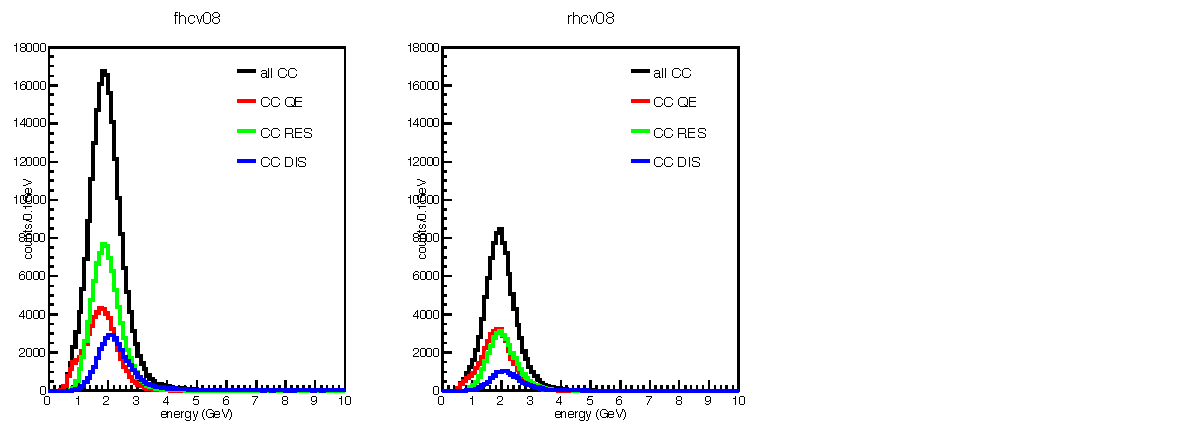
\includegraphics[width=.7\textwidth]{figures/2016/enspec_crop.pdf}
  \caption{Monte Carlo energy distribution broken down to interaction modes. Left: for $\nu_\mu$.  Right: for $\bar{\nu}_\mu$. Plots are normalized to 4e19 POT.}
  \label{fig:2016enspec}
\end{figure}

We can further ask if this short run is enough for a double differential cross section measurement, $\frac{d\sigma}{dp_\mu d\cos\theta_\mu}$, where $p_\mu$ is the muon momentum and $\theta_\mu$ is the muon angle with respect to the neutrino beam direction. This can be answered by dividing the phase space $(cos\theta_\mu, p_\mu)$ into a number of bins and see if most of the bins have enough statistics. The RHC result is shown in Figure~\ref{fig:2016rhc2dbin} while the FHC result is in Figure~\ref{fig:2016fhc2dbin}. From this comparison, doing a double differential measurement is perhaps also feasible.

\begin{figure}
  \centering
  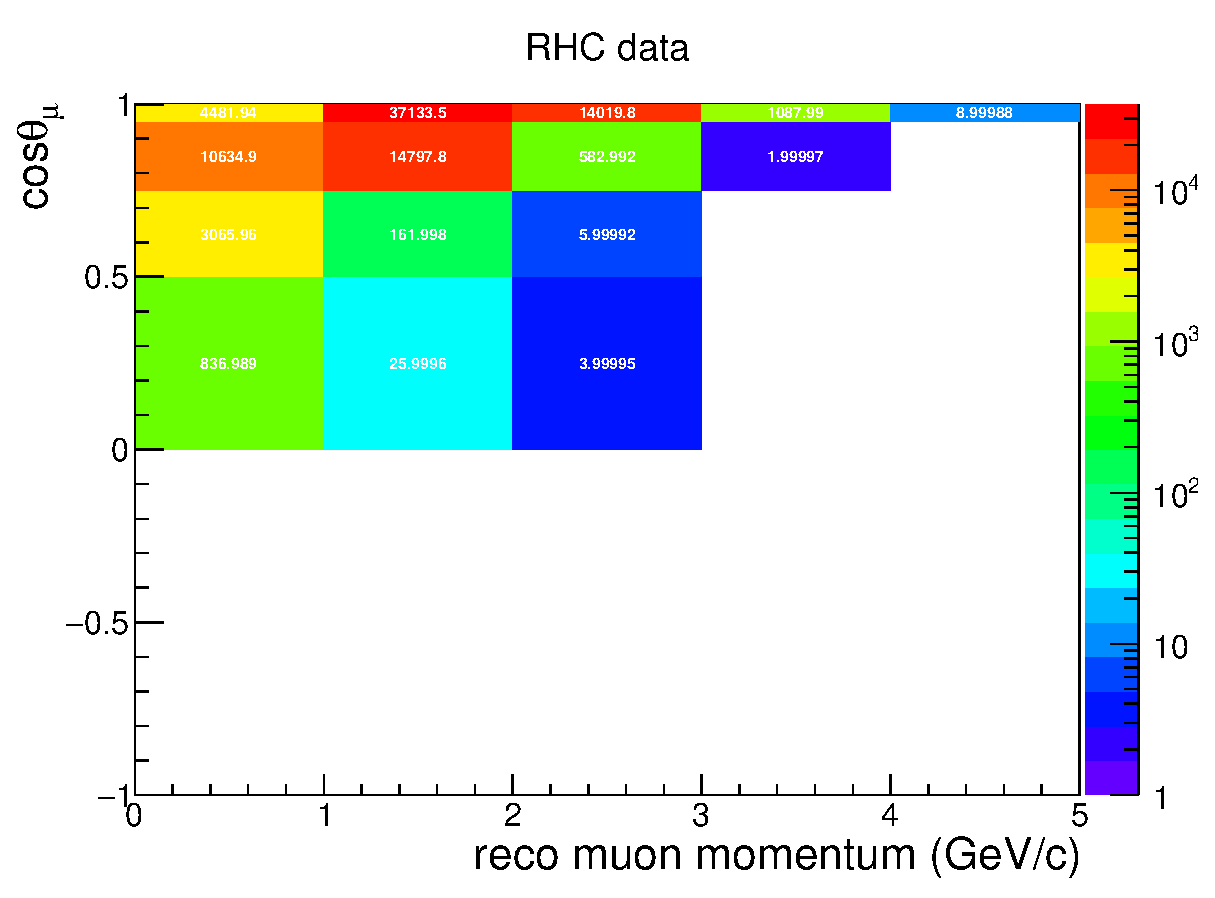
\includegraphics[width=.7\textwidth]{figures/2016/cosvspcoarse_text.eps}
  \caption{Number of events in each bin of the muon kinematic variables from RHC data.}
  \label{fig:2016rhc2dbin}
\end{figure}

\begin{figure}
  \centering
  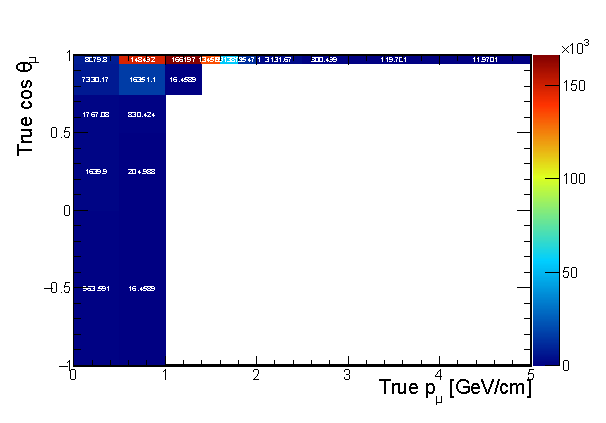
\includegraphics[width=.7\textwidth]{figures/2016/kanika_2d_binning.eps}
  \caption{Number of events in each bin of the muon kinematic variables from FHC MC.}
  \label{fig:2016fhc2dbin}
\end{figure}


\paragraph{\textbf{$\bar{\nu}_\mu$ selection optimization}}\hspace*{\fill}\\
I also tried to optimize the $\bar{\nu}_\mu$ selection criteria. One of the more straightforward selection to optimize is the ReMId PID variable. This is done by maximizing the figure-of-merit function, $\sqrt{\frac{S}{S+B}}$, where $S$ is the number of true $\bar{\nu}_\mu$ CC events selected by the PID, and $B$ is the number of background events selected. Figure~\ref{fig:2016rhcremid} shows that the maximum value happens at 0.65, meaning that $ReMId>0.65$ is the optimal cut associated with this FOM function.

\begin{figure}
  \centering
  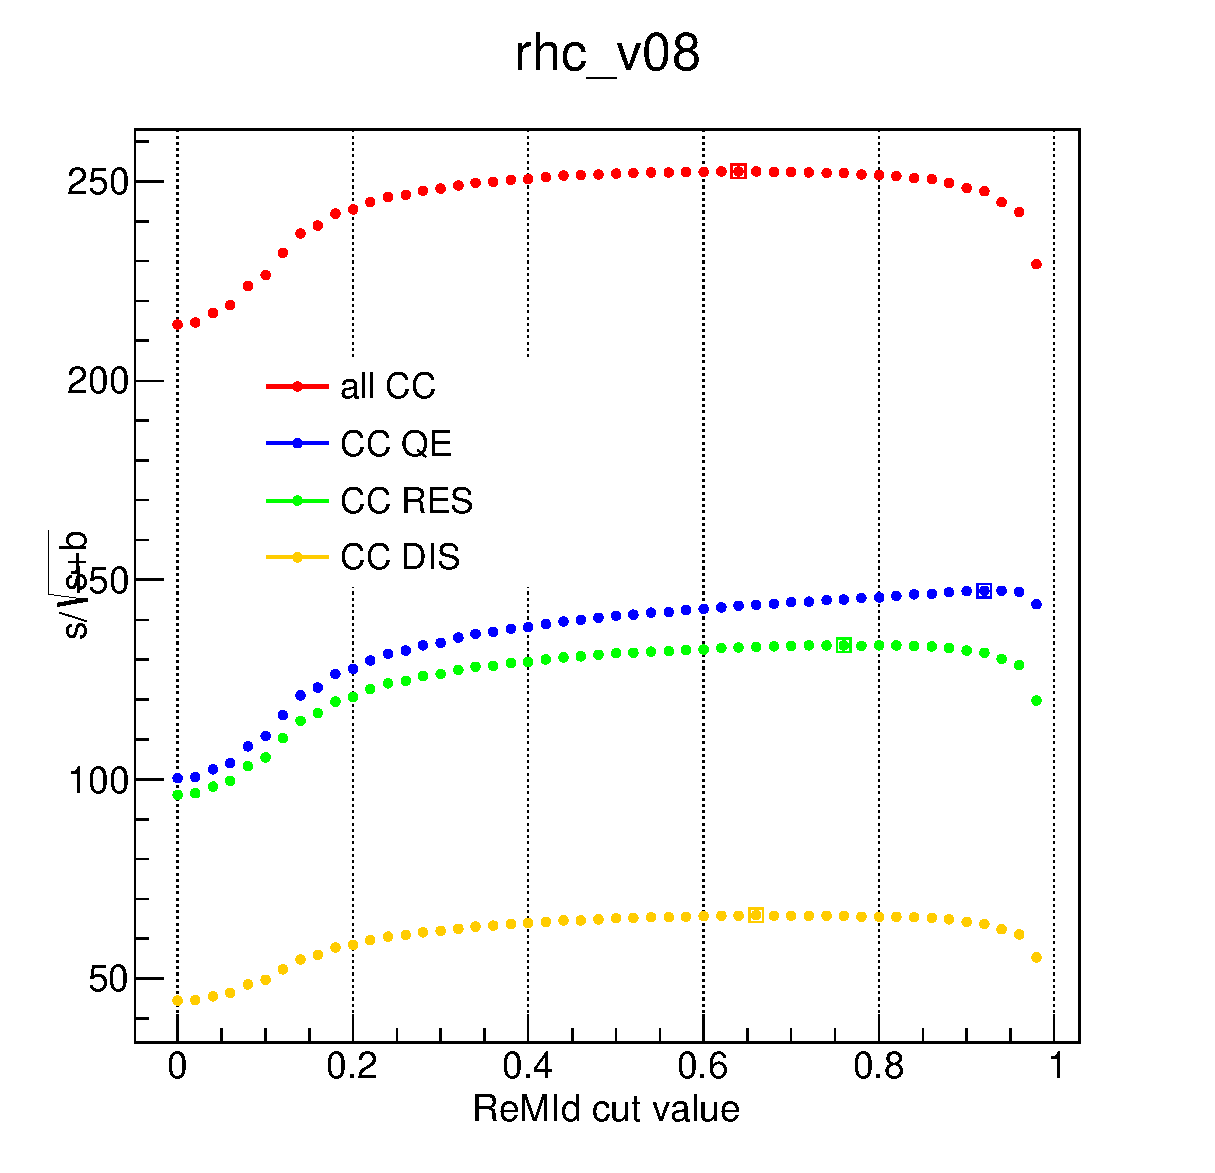
\includegraphics[width=.6\textwidth]{figures/2016/rhc_v08_remid.eps}
  \caption{FOM as a function of the ReMId cut value. Maximum happens at 0.65.}
  \label{fig:2016rhcremid}
\end{figure}

\paragraph{\textbf{Geant4 nuclear model systematics}}\hspace*{\fill}\\
One of the systematic uncertainties of the cross section measurement is caused by different Geant4 nuclear models used for generating the Monte Carlo sample. By switching to different nuclear models, we can quantify this effect. A preliminary study is shown in Figure~\ref{fig:2016truemu} and Figure~\ref{fig:2016truenu} for the true muon and neutrino energy, respectively. The variation is below $10\%$.

\begin{figure}
  \centering
  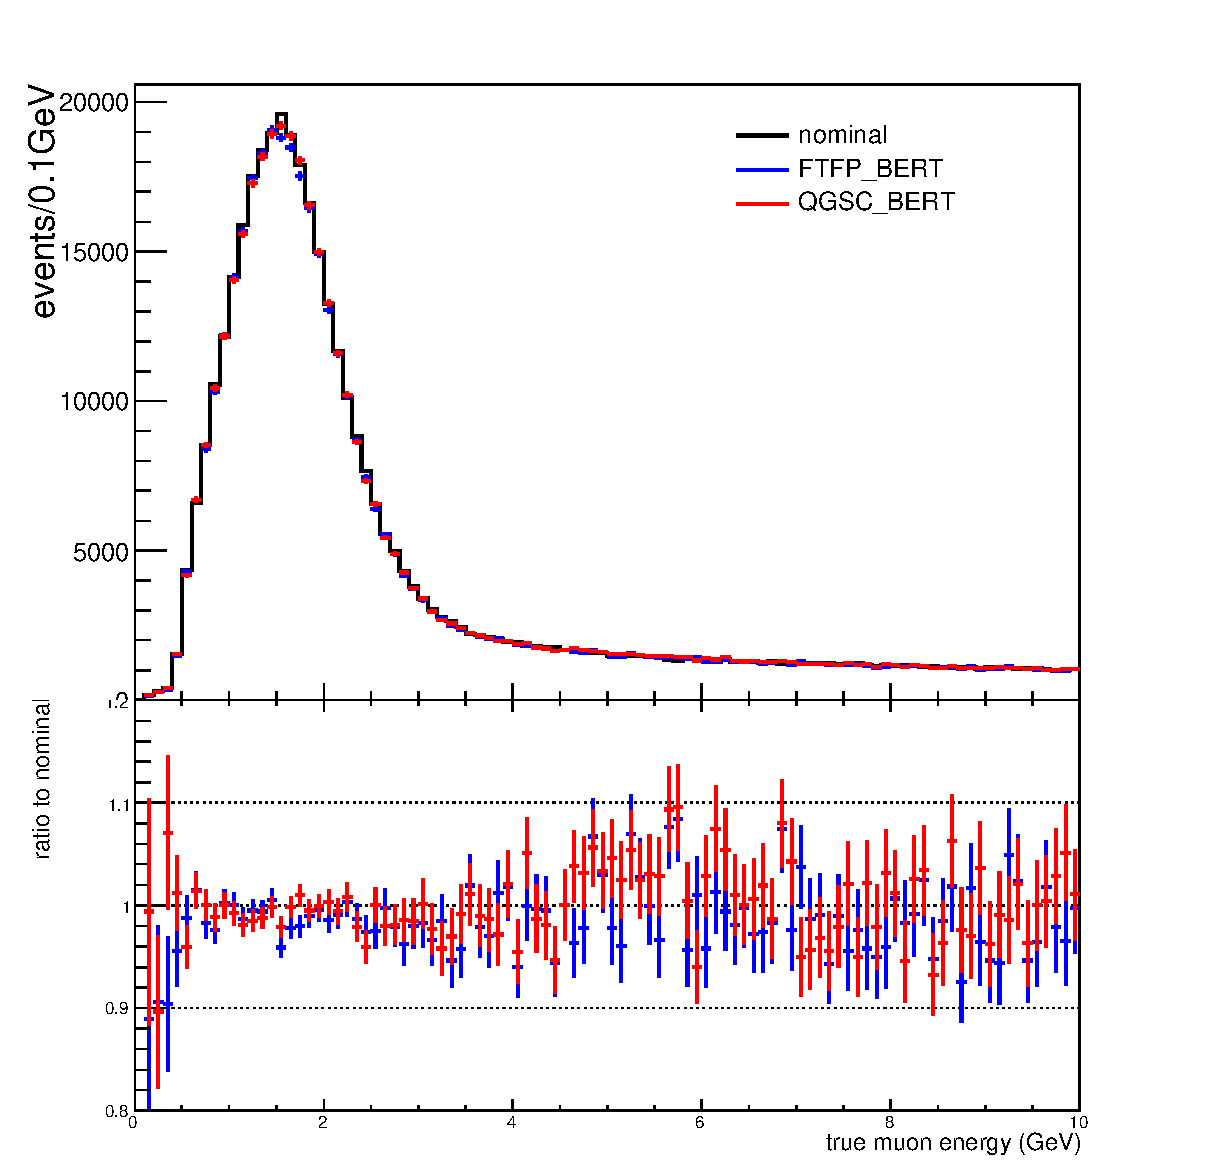
\includegraphics[width=.5\textwidth]{figures/2016/nuclear_model_mu.eps}
  \caption{True muon energy simulated with different Geant4 nuclear models.}
  \label{fig:2016truemu}
\end{figure}
\begin{figure}
  \centering
  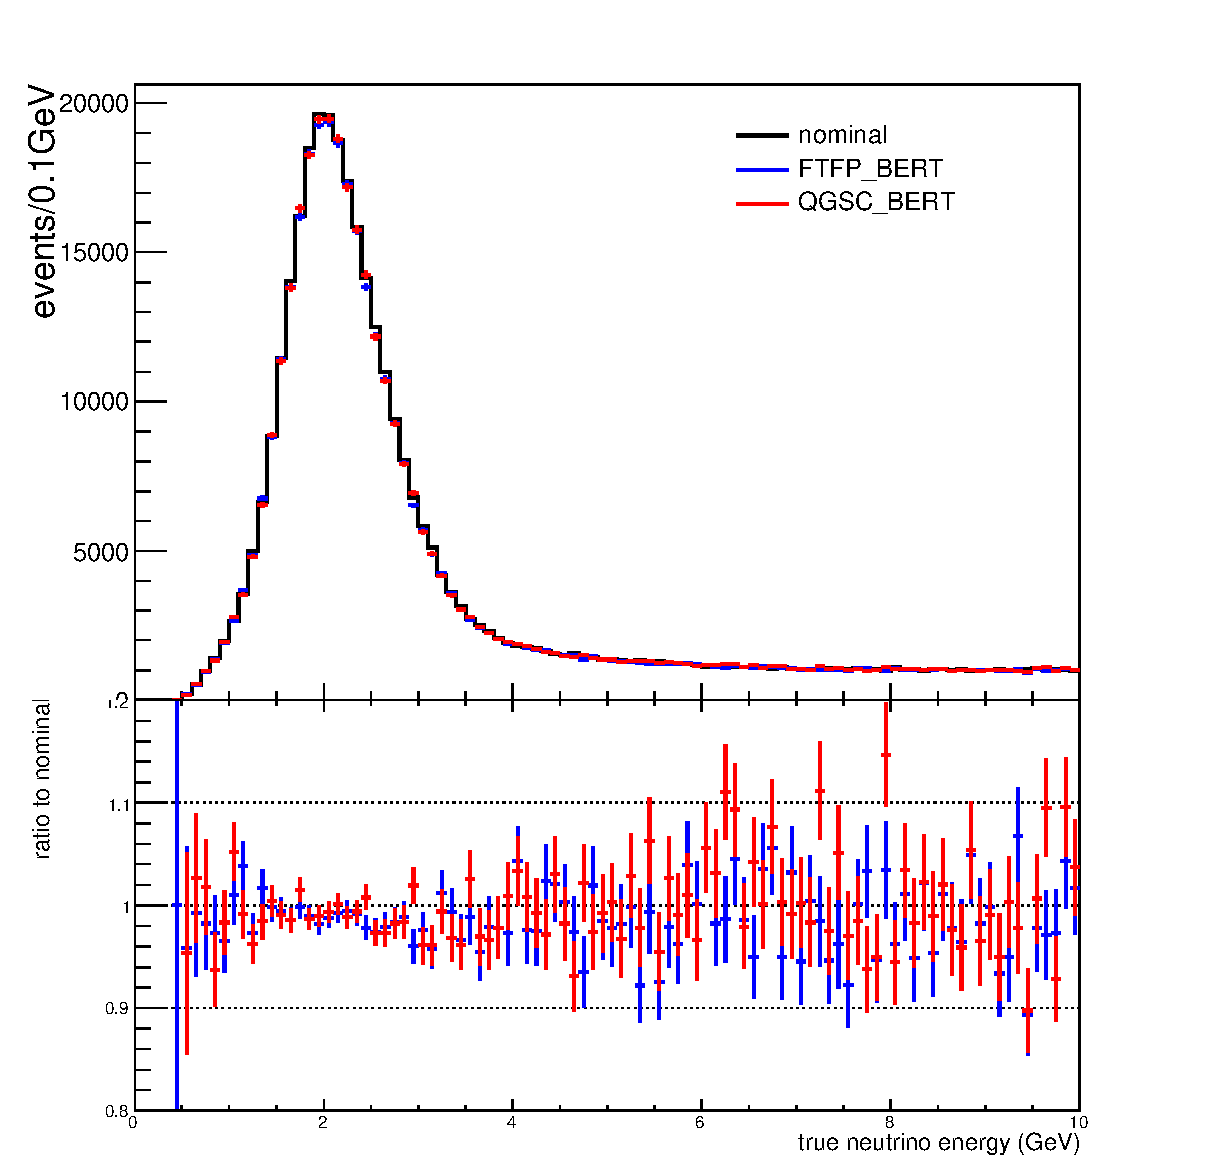
\includegraphics[width=.5\textwidth]{figures/2016/nuclear_model_nu.eps}
  \caption{True neutrino energy simulated with different Geant4 nuclear models.}
  \label{fig:2016truenu}
\end{figure}

\paragraph{\textbf{Rock muon rate for RHC}}\hspace*{\fill}\\
I generated a Monte Carlo sample with the "one interaction per spill`` mode, otherwise the generation will take much longer. After I finished generating the sample, I calculated the rock muon rate to be $\sim 7.75$ from the sample.

\paragraph{\textbf{Meson exchange current (MEC) effects for RHC}}\hspace*{\fill}\\
There is evidence that the MEC also has effects for RHC. Figure~\ref{fig:2016ehadscaled} shows a clear data excess for RHC results, and current MEC model for RHC cannot compensate the data access. More study is needed.

\begin{figure}
  \centering
  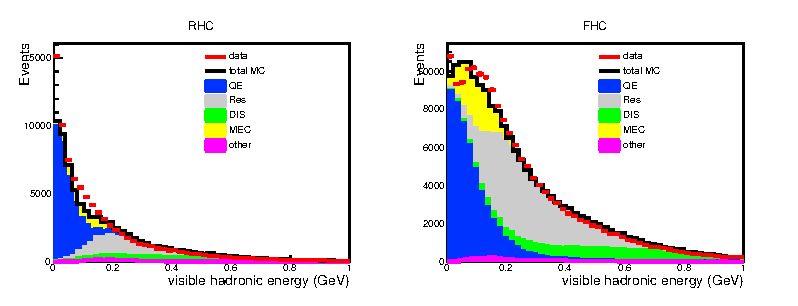
\includegraphics[width=.8\textwidth]{figures/2016/ehad_scaled.eps}
  \caption{Data and Monte Carlo comparison of the visible hadronic energy. The Monte Carlo is broken down to different interaction modes, and for RHC the resonant production is scaled down by 35\% and the deep inelastic scattering is scaled down by 15\%. The left plot is RHC, and the right plot is FHC.}
  \label{fig:2016ehadscaled}
\end{figure}


\subsubsection{Data Driven Trigger (DDT)}

\paragraph{\textbf{DDT code management and distribution}}\hspace*{\fill}\\
We plan to clean up unused code in the DDT code base. I will be watching over the integrity of DDT packages, validation of packages, and tagging and distributing new DDT releases. Switching back to the old SRT build system from MRB for building DDT code is also underway.

\paragraph{\textbf{DDT nearline}}\hspace*{\fill}\\
Right now DDT nearline is not working. I am working on incorporating the existing standalone DDT nearline into the nearline itself, which needs a code restructuring.

%%%%%%%%%%%%%%%%%%%%%%%%%%%%%%%%%%%%%%%%%%%%%%%%%%%%%%%%%%%%%%%%%%%%%%%%%%%%%%%%%%%%%%%%%%%%%%%%%%%%%%%%%%%%%%%%%%%%%%%%%%%%%%%%%%%%
% For 2015
\clearpage
\vspace*{\fill}
\begin{Huge}
\center{\textbf{Work in 2015}}
\end{Huge}
\vspace*{\fill}
\clearpage

\section{Work in 2015}

\subsection{DUNE}

\subsubsection{Comparison of Photon Detector Designs at CDDF}
We compared the performance of the photon detector designs from CSU and LSU. Detectors were put side by side in the Dewar at CDDF. Each detector has 2 SiPM channels. Figure~\ref{fig:cddfadc} shows the integrated ADC for the four SiPM channels. A threshold scan was done to set the threshold just above the pedestal peak. The detectors were irradiated by an $\alpha$ source and triggered at 0.5 photoelectron for each channel independently.

\begin{figure}
  \centering
  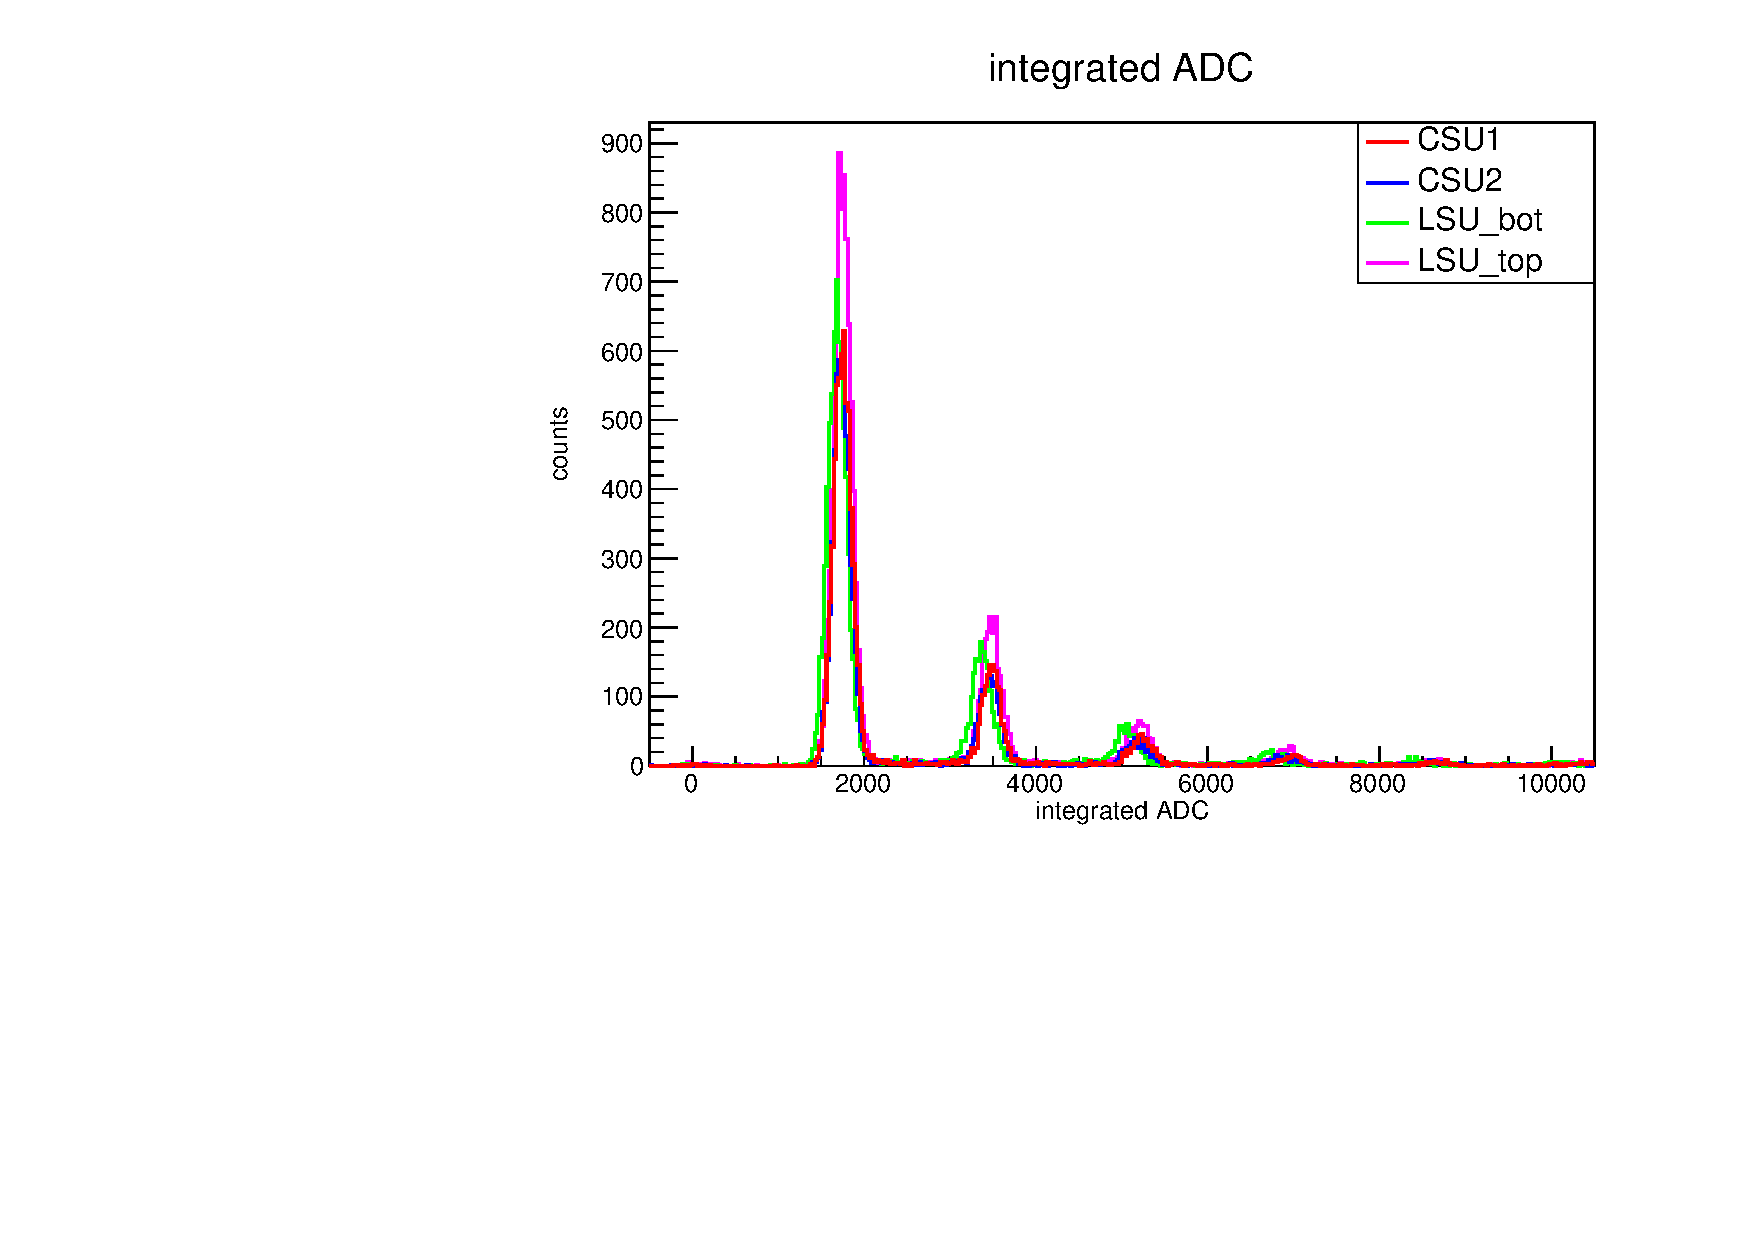
\includegraphics[angle=270,origin=c,width=.7\textwidth]{figures/2015/integratedADC.pdf}
  \caption{Integrated ADC for the four SiPM channels.}
  \label{fig:cddfadc}
\end{figure}

\begin{figure}
  \centering
  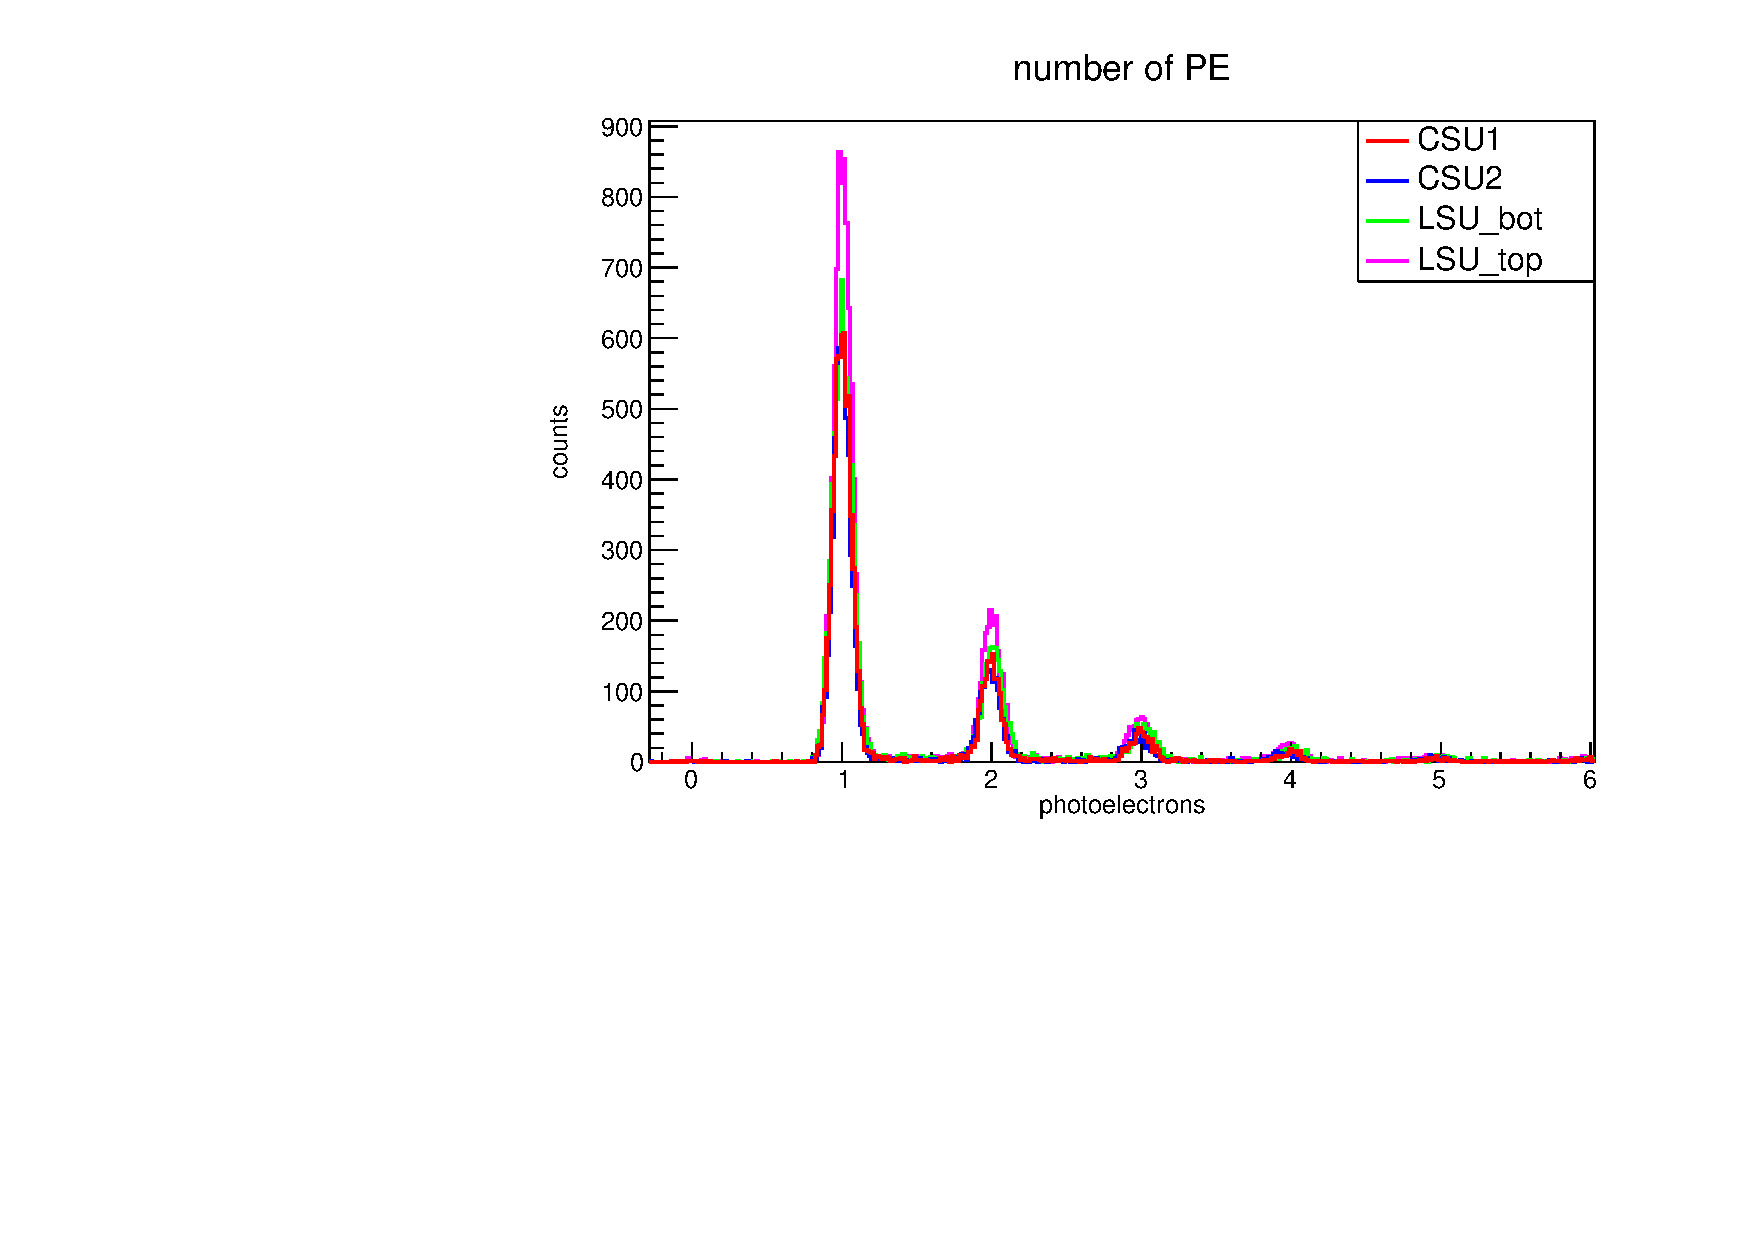
\includegraphics[angle=270,origin=c,width=.7\textwidth]{figures/2015/calibrated_spectra.pdf}
  \caption{ADC to photoelectron calibration for the four SiPM channels.}
  \label{fig:cddfcalibrated}
\end{figure}

\begin{figure}
  \centering
  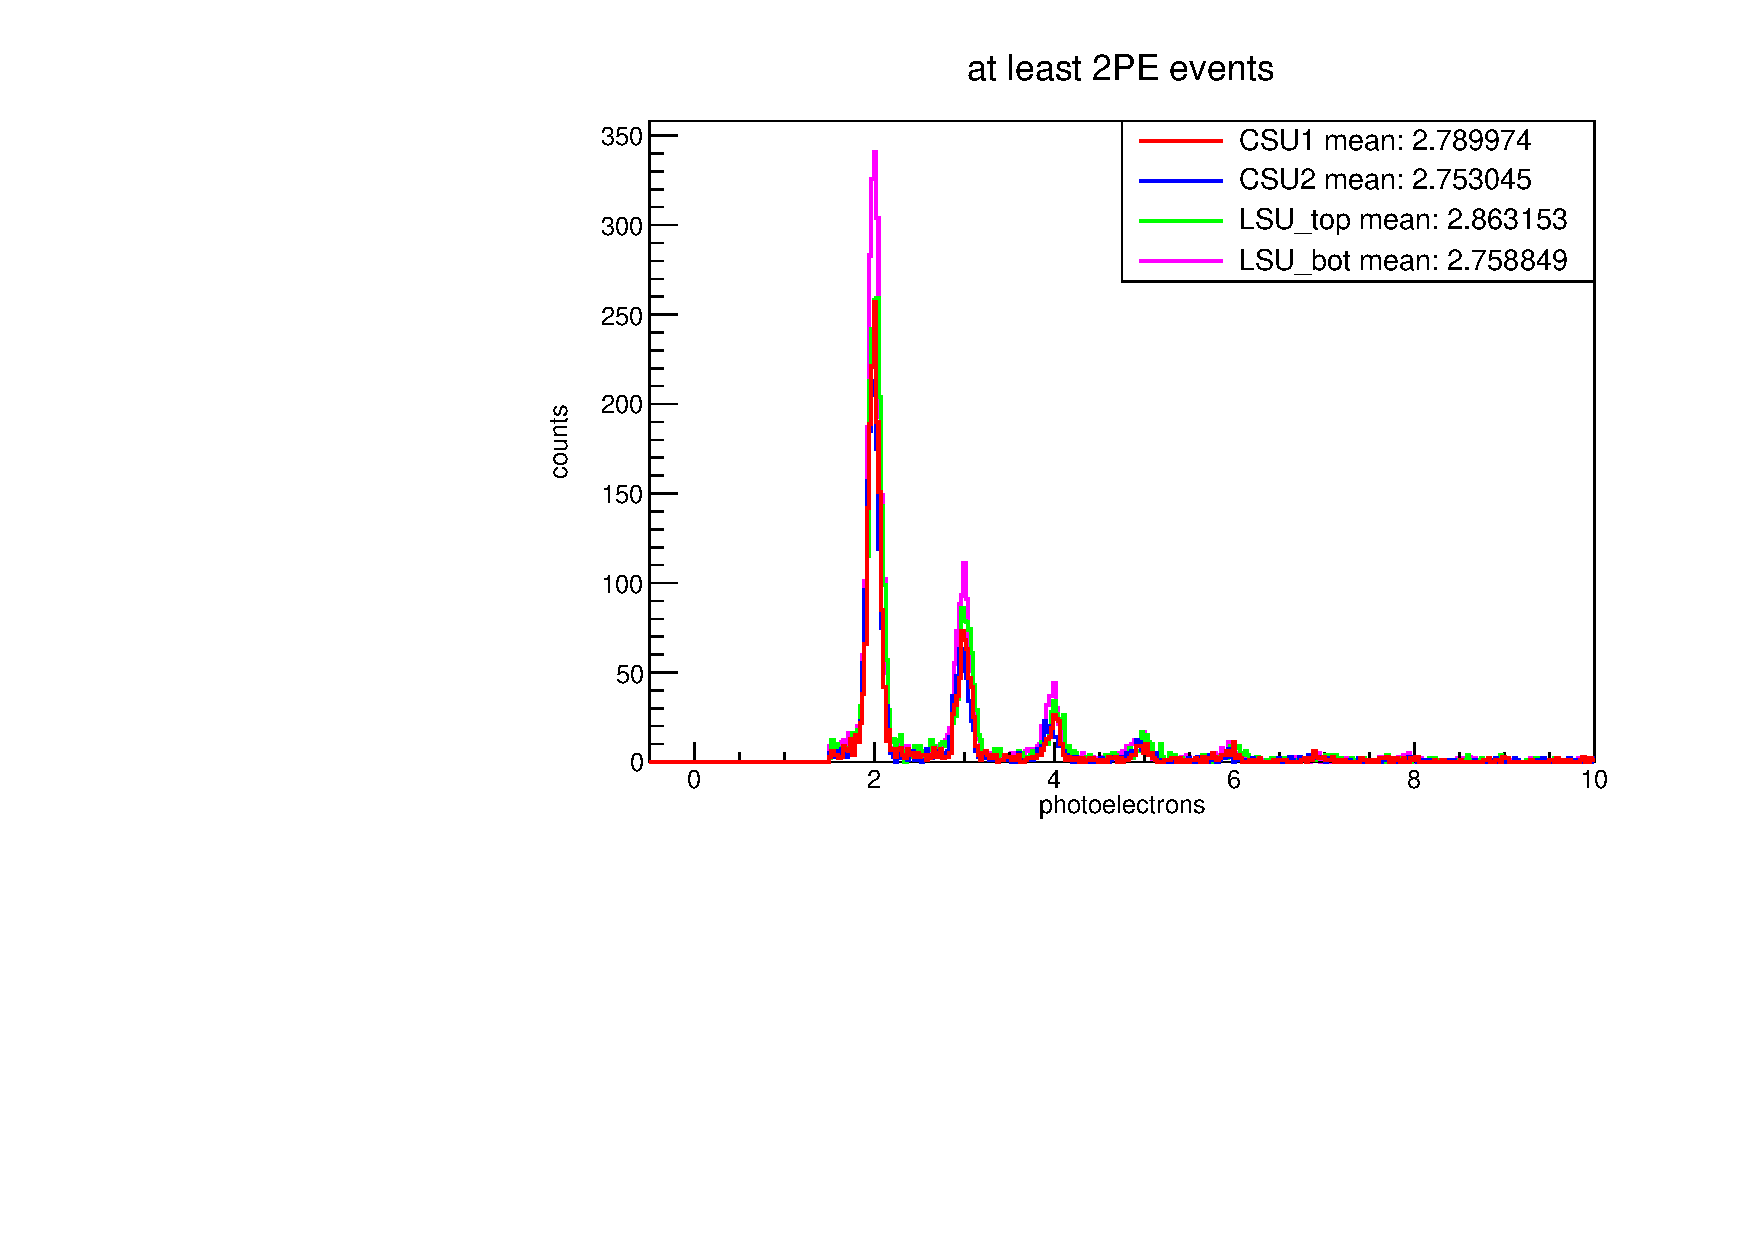
\includegraphics[angle=270,origin=c,width=.7\textwidth]{figures/2015/avgPE.pdf}
  \caption{Average light yield for at least 2 PEs for the four channels.}
  \label{fig:cddfly}
\end{figure}

Figure~\ref{fig:cddfcalibrated} shows calibrated photoelectron (PE) spectra for the four channels. The calibration was done by assigning the first peak to 1 PE, the second to 2 PE, etc.

Since the data showed a high trigger rate, the light yields were compared by excluding the single PE events. Figure~\ref{fig:cddfly} shows the average number of photoelectrons of events with at least 2 PEs. This figure shows the four channels have comparable light yield in this $\ge 2$ PE measure.

\subsubsection{Monitor Application for Voltage Readback of the SiPM Signal Processor}

CSU owns 2 SiPM Signal Processors (SSP). The SSP supplies high voltage to its 12 independent channels, and for each channel a readback register is in place for monitoring voltage in operation. A monitor application is developed to serve this purpose.

\subsubsection{Control Application for the LBNE Calibration Module}

This module is named after the former name of the experiment, LBNE. The LBNE Calibration Module (LCM) outputs calibration signals to 3 different calibration subsystem, namely, the Indiana University (IU) system, the TPC system, and the photon detector (PD) system. Figure~\ref{fig:pulser_pulse} shows sample pulses generated by the control application for the LCM. To facilitate the use of the control application, a simple GUI frontend is also provided as shown in Figure~\ref{fig:pulser_frontend}.

\begin{figure}
  \centering
  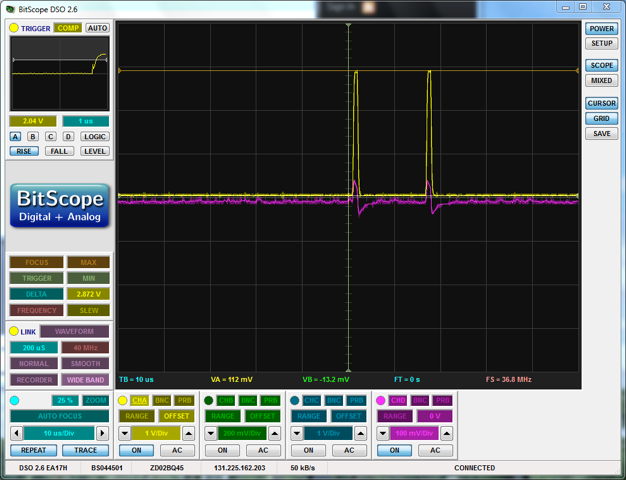
\includegraphics[width=.7\textwidth]{figures/2015/pulser.jpg}
  \caption{Sample pulses generated by the control application for the LCM.}
  \label{fig:pulser_pulse}
\end{figure}

\begin{figure}
  \centering
  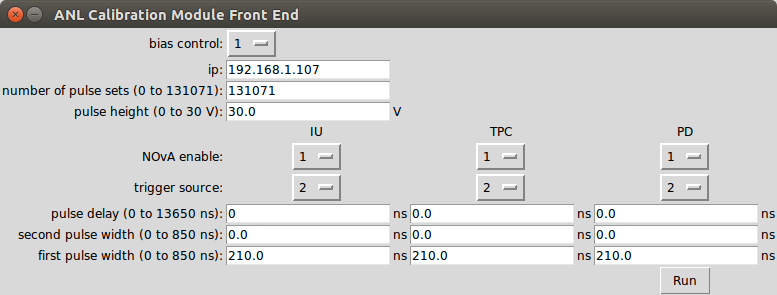
\includegraphics[width=.7\textwidth]{figures/2015/Screenshot_from_2015-09-23_10-49-58.png}
  \caption{A GUI frontend for the control application for the LCM.}
  \label{fig:pulser_frontend}
\end{figure}

\subsection[NOvA]{NO$\nu$A}

\subsubsection{Generation of Flat Monte Carlo Neutrino Spectrum}

The neutrino flux of the NuMI beam peaks at 2 GeV. The total interaction cross-section of neutrino is roughly $\sim E$, which at high energy is dominated by the deep inelastic scattering. The left plot in Figure~\ref{fig:NuMISpec} shows the total neutrino flux of the NuMI beam (the black histogram) from simulation. The right plot in Figure~\ref{fig:NuMISpec} is the neutrino event spectrum. The event spectrum is highly peaked around 2 GeV, leading to lack of statistics for particle identification (PID) training with neural network algorithms outside the peak range. There is need to warp the input neutrino flux to have a flat neutrino event spectrum for the PID training of the off-peak events. The idea is to make the input flux $\sim1/E$. Figure~\ref{fig:inverseEflux} shows the $1/E$ warped flux. Figure~\ref{fig:flatspec} is a sample output of the neutrino event spectrum gone through GENIE simulation with a $1/E$ input flux, which has an evenly distributed number of events in the interested energy range.

\begin{figure}
  \centering
  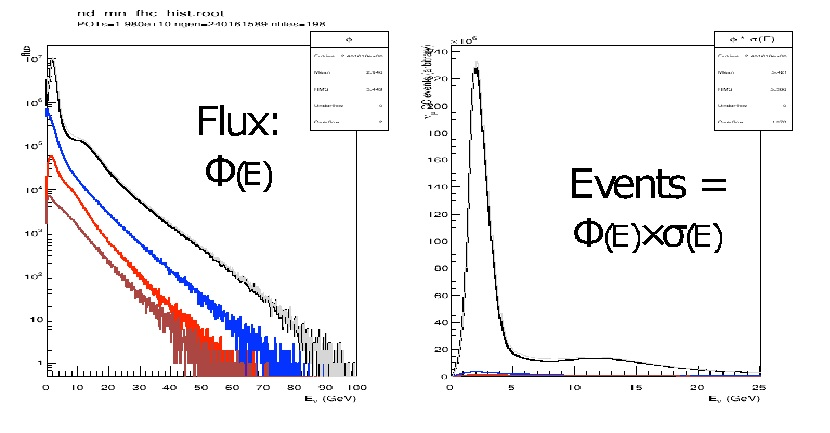
\includegraphics[width=.7\textwidth]{figures/2015/NuMI_spectrum.jpg}
  \caption{Left: The total neutrino flux of NuMI beam (black) and the fluxes of various components. Right: The neutrino event spectra for the corresponding fluxes.}
  \label{fig:NuMISpec}
\end{figure}

\begin{figure}
  \centering
  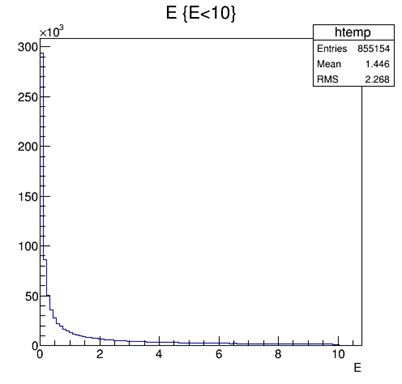
\includegraphics[width=.4\textwidth]{figures/2015/inverseEflux.png}
  \caption{The warped $1/E$ flux.}
  \label{fig:inverseEflux}
\end{figure}

\begin{figure}
  \centering
  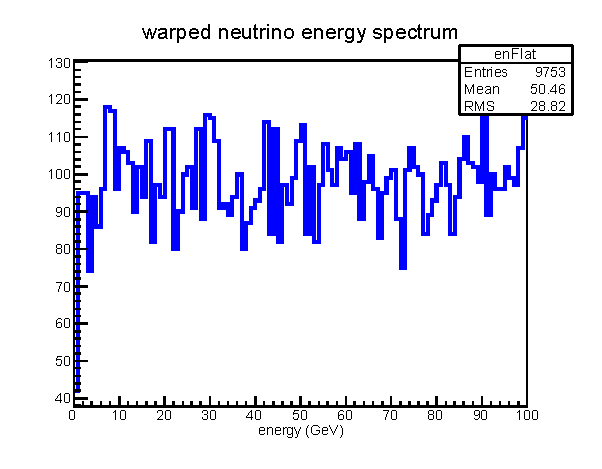
\includegraphics[width=.7\textwidth]{figures/2015/warped_event_spectrum.eps}
  \caption{The neutrino event spectrum with a $1/E$ input flux.}
  \label{fig:flatspec}
\end{figure}

\subsubsection[Numu on e Event Topology]{$\nu_\mu$ on e event topology}

$\nu_\mu-e$ scattering is one of the simplest processes whose cross-section can be calculated very accurately. Therefore these events can be used for constraining the NuMI flux. The characteristic feature of the $\nu_\mu-e$ events leaving in the detector is a 1-prong electromagnetic shower in the very forward direction.  We used the near detector MC data to check how well our current reconstruction algorithms work for $\nu_\mu-e$ scattering events. A sample event where the current reconstruction algorithms reconstruct successfully as a 1-prong event is given in Figure~\ref{fig:oneprong}. However there are also events in which the number of the reconstructed prongs is more than one, such as that shown in Figure~\ref{fig:multiprong}. This is because current algorithms pull the vertex downstream into the shower, leaving 2 back-to-back prongs. The proportion of events for which current algorithms perform well is about $70\%$, while the proportion of the incorrectly reconstructed events is about $30\%$, leaving room for improvements.

\begin{figure}
  \centering
  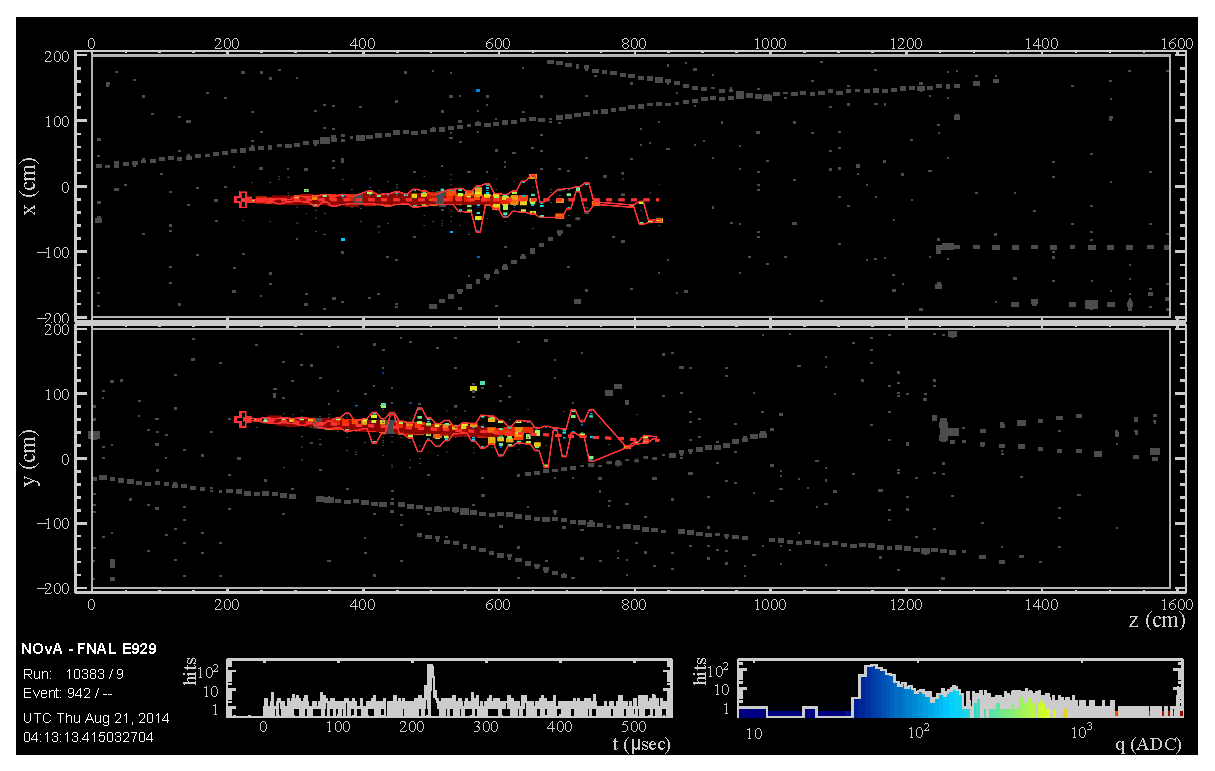
\includegraphics[width=\textwidth]{figures/2015/nelastic1npng3d1.eps}
  \caption{A $\nu_\mu$ on $e$ event where the current reconstruction algorithms reconstruct successfully as a 1-prong event. The upper plot is the top view of the NO$\nu$A near detector, while the bottom is the side view of it.}
  \label{fig:oneprong}
\end{figure}

\begin{figure}
  \centering
  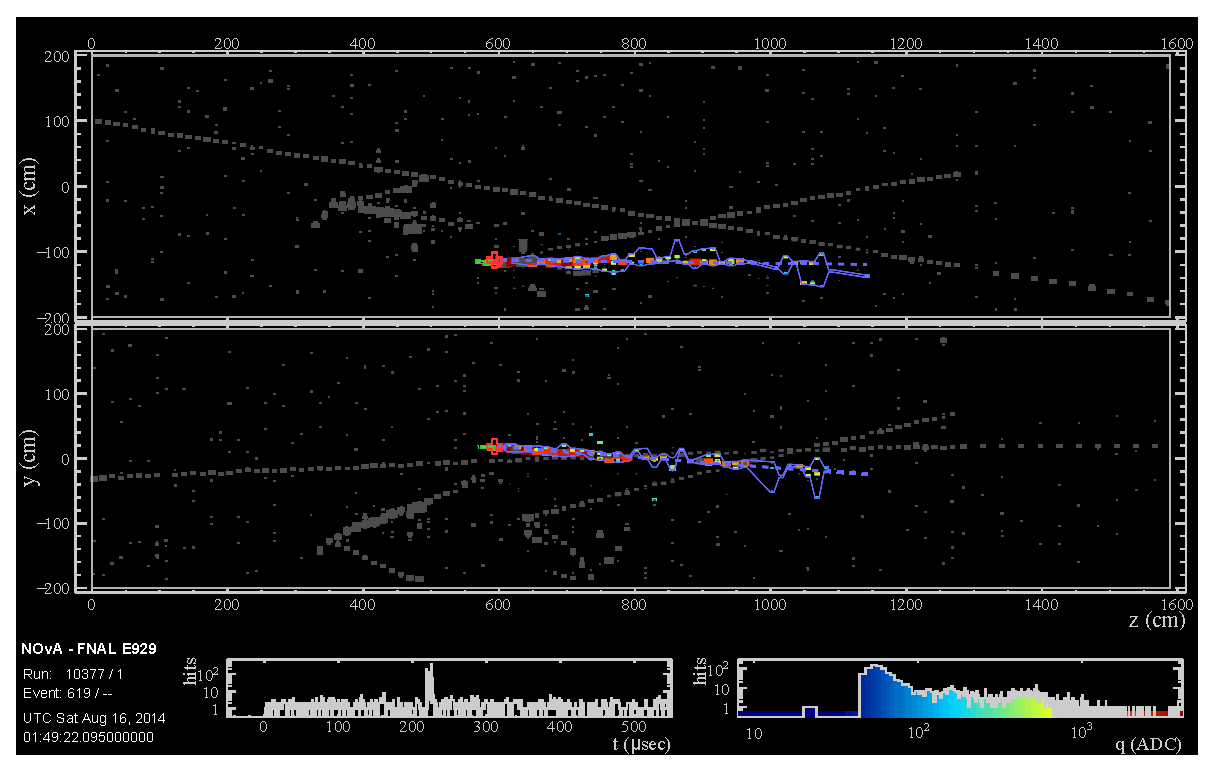
\includegraphics[width=\textwidth]{figures/2015/nelastic1npng3d1+.eps}
  \caption{A $\nu_\mu$ on $e$ event where the current reconstruction algorithms reconstruct incorrectly as a multi-prong event. The hollow cross indicates the reconstructed vertex where the interaction happens. Current algorithms pull the vertex downstream into the shower, leaving 2 back-to-back prongs.}
  \label{fig:multiprong}
\end{figure}

%\section*{References}
%\begin{thebibliography}{10}
%\bibitem{ref1} J.~Doe, Article name, \textit{Phys. Rev. Lett.}
%
%\bibitem{ref2} J.~Doe, J. Smith, Other article name, \textit{Phys. Rev. Lett.}
%
%\bibitem{web} \href{http://www.google.pl}{www.google.pl}
%\end{thebibliography}

\end{document}

